    MPI (\textit{Message-Passing Interface}) ist eine Spezifikation für den Nachrichtenaustausch eines verteilten Systems. MPI richtet sich hauptsächlich nach dem 
    \textit{Message-Passing-Modell} (siehe \autoref{sec:mpm}).
    Erweitert wird das ``klassische'' Message-Passing-Modell unter anderem durch kollektive Kommunikationsmöglichkeiten, Remote-Speicherzugriff und parallele I/O-Operationen.
    Als Interface bietet MPI selbst keine Implementierung des Standards, sondern beschreibt Methoden und ihre Semantik.
    
    Das Ziel von MPI ist es, einen Standard für Programme zu liefern, die sich des Message-Passing-Modells bedienen, und somit zu Effizienz, Portabilität und Flexibilität
    beizutragen. \citep{mpiv31}
    
    \subsection{Geschichte}
      Bereits vor 1992 gab es Bibliotheken für paralleles Rechnen. Jedoch gab es keinen einheitlichen Standard und die meisten Bibliotheken waren systemspezifisch,
      sodass das Portieren von Programmen auf ein anderes System zumindest eine aufwendige Aufgabe war. Auch die Ansätze der Bibliotheken unterschieden sich teilweise
      stark. Ein weit verbreiteter Ansatz war allerdings das Message-Passing-Model, bei dem die verteilten Prozessteile Nachrichten austauschen, um eine gemeinsame
      Aufgabe zu erfüllen.\citep{mpitut}
      
      Am 29. und 30. April 1992 begann mit dem \textit{Workshop on Standards for Message-Passing in a Distributed Memory Environment} am \textit{Center for Research on Parallel 
      Computing} in Williamsburg (Virginia) ein Prozess zur Standardisierung des Message-Passing-Ansatzes \citep{workshop}. Hier wurden die essentiellen Bestandteile eines 
      standardisierten Message-Passing-Interfaces diskutiert. An diesem Prozess waren rund 60 Personen von 40 verschiedenen Organisationen beteiligt, darunter die bedeutendsten
      Anbieter von Parallelrechnern sowie Forscher aus Universitäten, staatlichen Laboren und der Industrie. Die Ergebnisse wurden zunächst in einem vorläufigen Entwurf im
      November 1992 und schließlich in revidierter Fassung in einem Proposal, bekannt als MPI-1, veröffentlicht. \citep{mpi1}
      
      Eine Hauptabsicht von MPI-1 war es, erst einmal den ``Ball in's Rollen zu bringen'' und eine Diskussion anzuregen. Daher beschäftigte es sich noch hauptsächlich
      mit Point-to-Point-Kommunikation. Zu diesem Zeitpunkt war MPI weder thread safe, noch bot es Methoden zur kollektiven Kommunikation. Aktuell liegt MPI in der Version 3.1
      vor und bietet neben der Point-to-Point-Kommunikation auch kollektive Routinen, nicht-blockierende Methoden, automatische Puffer-Verwaltung und vieles mehr. \citep{mpiv31}
      
      \TODO{Umsetzung in C und Fortran \\* später auch bindings für c++}
      
    \subsection{Point-to-Point-Kommunikation}
    \label{sek:ptpkom}
    Die Point-to-Point-Kommunikation ist das durch das Message-Passing-Modell beschriebene Herzstück von MPI.  
    Die Standardmethoden in C-Syntax sind:
    \begin{lstlisting}[language=C, label=lst:p2p_standard, caption={Die Syntax der standard Sende- und Empfangsoperationen}, numbers=none]
	MPI_Send(
	  void* data,
	  int count,
	  MPI_Datatype datatype,
	  int destination,
	  int tag,
	  MPI_Comm communicator)

	MPI_Recv(
	  void* data,
	  int count,
	  MPI_Datatype datatype,
	  int source,
	  int tag,
	  MPI_Comm communicator,
	  MPI_Status* status)

    \end{lstlisting}
    
    Jede Nachricht besteht aus einem Daten-Teil sowie einem \textit{Umschlag} (engl.: envelope). Der Daten-Teil beinhaltet die Daten, die vom Sende- in den Empfangspuffer kopiert
    werden sollen (\code{void* data}), deren Anzahl (\code{int count}) sowie den Datentyp der zu sendenden Elemente (\code{MPI\_Datatype datatype}). \citep{mpiv31}
    
    Der Umschlag besteht aus:
    \begin{labeling}{Kennzeichnung}
     \item[Sender] Dieser bei der Point-to-Point-Kommunikation automatisch hinzugefügt, muss aber bei der kollektiven Kommunikation explizit angegeben werden (vgl.: \autoref{sek:kolkom}).
     \item[Empfänger] Jeder Prozess im Kommunikator hat eine eindeutige Nummer. Über diese Nummer (\code{int destination}) wird der Empfänger festgelegt.
     \item[Kennzeichnung] Eine Kennzeichnung (engl.: tag) kann zur Differenzierung der Nachrichten eingesetzt werden (\code{int tag}).
     \item[Kommunikator] Der \code{MPI\_Comm communicator} spezifiziert eine Menge von $p$ Prozessen, die sich diesen Kommunikator teilen. Die \textit{Prozessgruppe} ist geordnet und
			 die Prozesse sind durch ihren Rang \code{destination} $\in \nullhaken{p-1}$ innerhalb der Gruppe spezifiziert.
    \end{labeling}
    Diese Informationen ermöglichen es, Nachrichten voneinander unterscheiden und selektiv empfangen zu können. Der zugehörige Empfängeraufruf muss genau zum Sendeaufruf
    passen. \citep{mpiv31}
    
    \code{MPI\_Status* status} dient dem empfangenden Prozess dazu eventuelle Fehler zu erhalten. Dies ist besonders dann wichtig, wenn der Sender oder die Kennzeichnung,
    zum Beispiel auf Grund der Nutzung von Wildcards, nicht bekannt ist. Der Datentyp \code{MPI_Status} enthält dazu die Member \code{MPI_SOURCE}, \code{MPI_TAG} und \code{MPI_ERROR}.
    \citep{mpiv31}
    
    \begin{table}
      \begin{tabular}{|c|c|c|}
	\hline
	\textbf{Kommunikationsmodus}&\textbf{blockierende Methode}&\textbf{nicht-blockierende Methode}\\
	\hline
	Standard		    &MPI\_Send			  &MPI\_Isend			      \\
	\hline
	Synchro                     &MPI\_Ssend                   &MPI\_Issend                        \\
	\hline
	Ready                       &MPI\_Rsend                   &MPI\_Irsend                        \\
	\hline
	Buffered                    &MPI\_Bsend                   &MPI\_Ibsend                        \\
	\hline
	                            &MPI\_Recv                    &MPI\_Irecv                         \\
	\hline
      \end{tabular}
    \caption{MPIs Point-to-Point-Kommunikationsvarianten (Quelle: \citet{mpi_p2p})}
    \label{tab:p2p_comm}
    \end{table}
    
    Bei den in \autoref{lst:p2p_standard} dargestellten Standard-Point-to-Point-Methoden handelt es sich um blockierende Operationen. Das heißt, dass das Programm aus \code{MPI\_Send} 
    erst zurückkehrt, wenn sicher ist, dass die gesendeten Daten wieder verändert werden dürfen. Entweder, weil sie in einen temporären Systempuffer, oder weil sie bereits in den 
    Empfängerspeicher übertragen wurden.
    Dies kann bei manchen Programmen zu viel Wartezeit führen, andere benötigen eventuell mehr Sicherheit im Ablauf. Daher bietet MPI Variationen dieser Standard-Sendeoperation an. 
    Diese sind in \autoref{tab:p2p_comm} aufgelistet und werden im Folgenden kurz erläutert.
    
    Beim synchronen Senden wird, wie in \autoref{fig:send_var}\hyperref[fig:sync_send]{.(a)} dargestellt, zunächst vom sendenden Prozess eine ``Ready to send''-Mitteilung verschickt. Auf 
    diese Antwortet der empfangende Prozess mit einer ``Ready to receive''-Mitteilung. Im Anschluss findet das Senden und Empfangen der Daten statt. Durch dieses Vorgehen müssen die Prozesse
    aber gegebenenfalls auf einander warten. Die Wartezeit ist in der Abbildung dunkel eingefärbt. Dafür wird aber nicht nur sichergestellt, dass die gesendeten Daten verändert werden dürfen,
    sondern auch, dass der Empfänger-Prozess zumindest damit begonnen hat die Daten auch zu empfangen. \citep{mpi_p2p, mpiv31}
    
    Das Ready-Send sieht wie eine einfachere synchrone Sende-Variante aus (vgl. \autoref{fig:send_var}\hyperref[fig:ready_send]{.(b)}), ist aber restriktiver. Die Methoden \code{MPI\_Rsend}
    beziehungsweise \code{MPI\_Irsend} erwarten, dass die ``Ready to receive''-Mitteilung bereits geschickt wurde, wenn sie aufgerufen werden. Nur wenn diese Mitteilung bereits eingetroffen
    ist, werden die Daten auch gesendet, ansonsten wird ein Fehler gemeldet. Diese Methode soll den System-Overhead durch Sendeoperationen und Synchronisation minimieren. Es wird jedoch 
    dazu geraten diese Methode nur zu verwenden, wenn die zeitliche Abfolge garantiert ist. \citep{mpi_p2p, mpiv31}
    
    Beim Buffered-Send werden die Daten in einem gesonderten Puffer zwischengespeichert. Dies führt durch das zusätzliche Kopieren gegebenenfalls zu weiterem Overhead, dafür kann der 
    Prozess, wie in \autoref{fig:send_var}\hyperref[fig:buff_send]{.(c)} zu erkennen, im Anschluss an den Kopiervorgang seine Arbeit fortsetzen und auch den Sendepuffer bereits verändern. 
    Die eigentliche Sendeoperation wird dann zu einem späteren Zeitpunkt nach der ``Ready to receive''-Mitteilung des Empfängers durchgeführt. Der Puffer zum Zwischenspeichern muss allerdings 
    auch durch den Nutzer zur Verfügung gestellt werden und wird nicht automatisch durch das System verwaltet. \citep{mpi_p2p, mpiv31}
    
    Bei allen blockierenden Methoden können Deadlocks auftreten. Diese können beispielsweise entstehen, wenn zwei Prozesse Daten austauschen wollen, jedoch beide mit einer Sendeoperation
    beginnen, die nicht zurückkehrt, bevor nicht auch das Empfangen der Daten begonnen wurde. Beide Prozesse werden niemals beginnen Daten zu empfangen und werden somit auch
    nie aus dem Senden zurückkehren. Abhilfe können die nicht-blockierenden Methoden liefern.
    
    Die nicht-blockierenden Methoden bestehen grundsätzlich aus zwei Aufrufen. Einer Initialisierung des Sendens/Empfangens, ohne dass auf dessen Ausführung gewartet wird, und
    einer Abschlussmethode, wie \code{MPI\_Wait}, \code{MPI\_Probe} oder \code{MPI\_Test}. Dies ermöglicht es dem sendenden und dem empfangenden Prozess weitere Arbeiten auszuführen,
    um so möglichst Wartezeiten zu vermeiden beziehungsweise produktiv zu nutzen. Allerdings sollten weder der Sende- noch der Empfangspuffer zwischen Initialisierung und Abschluss
    verändert werden. \citep{mpi_p2p, mpiv31}
    
    \begin{figure}[t]
      \begin{subfigure}[c]{0.53\textwidth}
	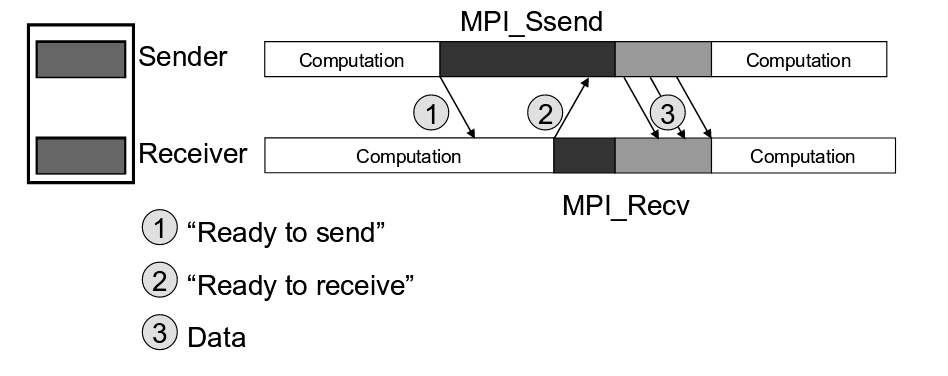
\includegraphics[width=0.9\textwidth]{img/SyncSend_gray.png}
	\subcaption{Ablauf der synchronen Sendeoperation.}
	\label{fig:sync_send}
      \end{subfigure}
      \begin{subfigure}[c]{0.45\textwidth}
	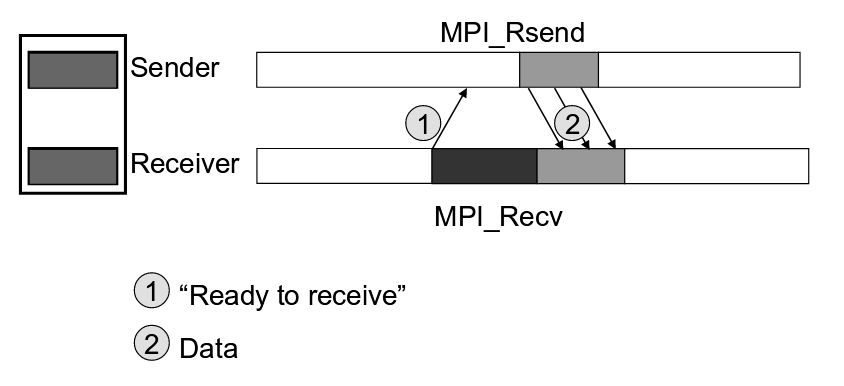
\includegraphics[width=0.9\textwidth]{img/ReadySend_gray.png}
	\subcaption{Ablauf der Ready-Send-Operation.}
	\label{fig:ready_send}
      \end{subfigure}
      \begin{subfigure}[c]{0.5\textwidth}
	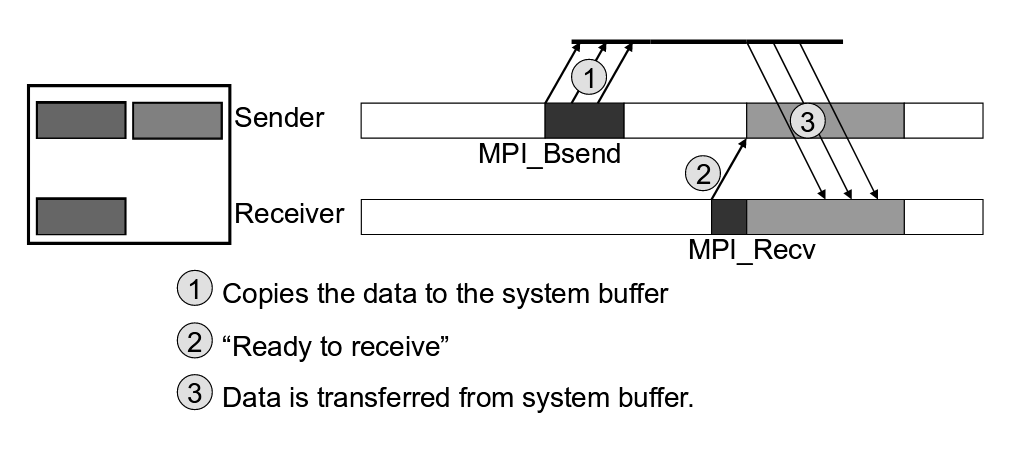
\includegraphics[width=0.9\textwidth]{img/BufferedSend_gray.png}
	\subcaption{Ablauf der gepufferten Sendeoperation.}
	\label{fig:buff_send}
      \end{subfigure}
      \caption{Quelle: \citet{mpi_p2p}}
      \label{fig:send_var}
    \end{figure}
    
%     \begin{figure}[p]
%       \begin{subfigure}[c]{0.9\textwidth}
% 	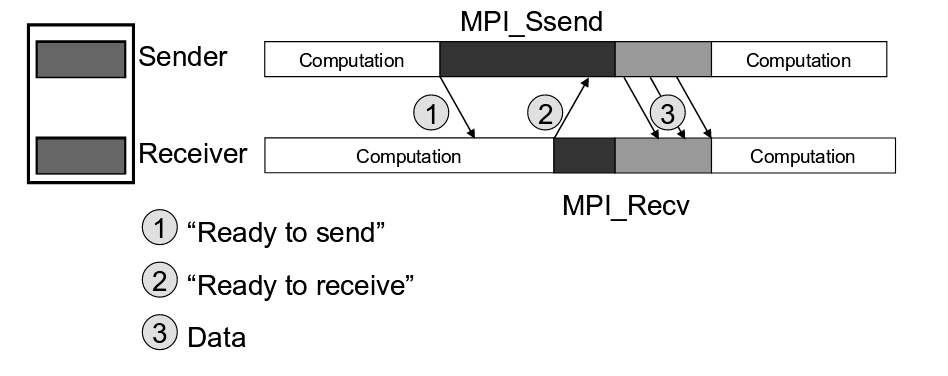
\includegraphics[width=0.9\textwidth]{img/SyncSend_gray.png}
% 	\subcaption{Ablauf der synchronen Sendeoperation.}
% 	\label{fig:sync_send}
%       \end{subfigure}
%       \begin{subfigure}[c]{0.9\textwidth}
% 	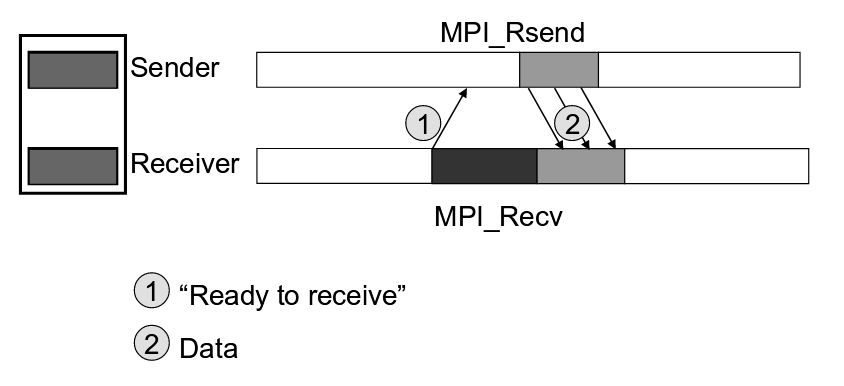
\includegraphics[width=0.9\textwidth]{img/ReadySend_gray.png}
% 	\subcaption{Ablauf der Ready-Send-Operation.}
% 	\label{fig:ready_send}
%       \end{subfigure}
%       \begin{subfigure}[c]{0.9\textwidth}
% 	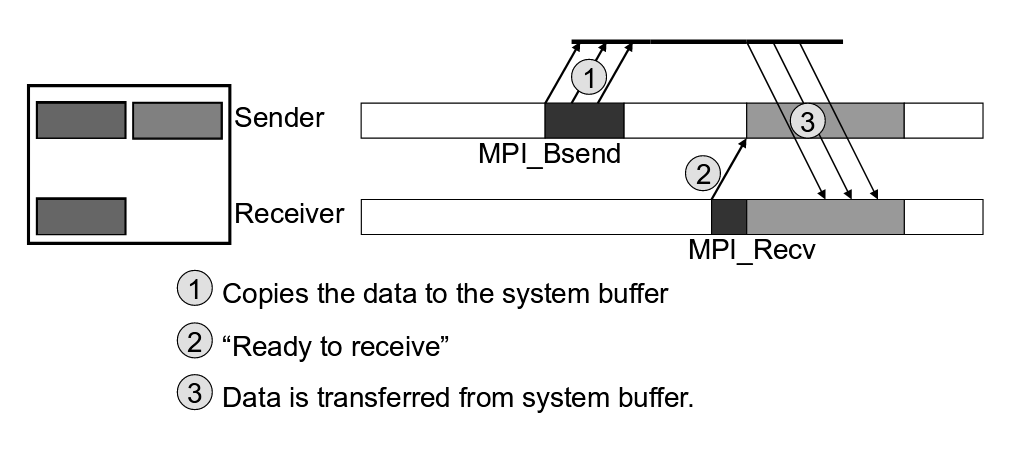
\includegraphics[width=0.9\textwidth]{img/BufferedSend_gray.png}
% 	\subcaption{Ablauf der gepufferten Sendeoperation.}
% 	\label{fig:buff_send}
%       \end{subfigure}
%       \caption{Quelle: \citet{mpi_p2p}}
%       \label{fig:send_var}
%     \end{figure}
%     \clearpage
      
    \subsection{Kollektive Kommunikation}
    \label{sek:kolkom}
    
    \begin{center}
      \begin{figure}[b]
      \centering
      \begin{subfigure}{0.9\textwidth}
      \begin{lstlisting}[language=C, label=lst:bcast, caption={Die Syntax von \code{MPI\_Bcast}}, numbers=none]
	MPI_Bcast(
	  void* data,
	  int count,
	  MPI_Datatype datatype,
	  int root,
	  MPI_Comm communicator)
      \end{lstlisting}
      \end{subfigure}
      \end{figure}
      
      \begin{figure}[b]
	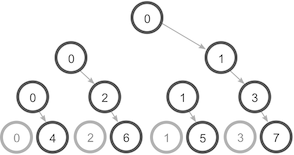
\includegraphics{img/bcast_tree_gray.png}
	\caption{Mögliche Verteilung der Daten durch \code{MPI\_Bcast}. (Quelle: \citet{mpitut})}
	\label{fig:bcast_tree}
      \end{figure}
      \end{center}
      
      \begin{figure}[t]
      \begin{subfigure}{0.9\textwidth}
      \begin{lstlisting}[language=C, label=lst:a2a, caption={Die Syntax von \code{MPI\_Alltoallv}}, numbers=none]
	int MPI_Alltoallv(
	  const void* sendbuffer,
	  const int sendcounts[], 
	  const int senddispls[], 
	  MPI_Datatype sendtype, 
	  void* recvbuffer, 
	  const int recvcounts[], 
	  const int recvdispls[], 
	  MPI_Datatype recvtype, 
	  MPI_Comm comm)
      \end{lstlisting}
      \end{subfigure}
      \end{figure}
      Zusätzlich zur klassischen Point-to-Point-Kommuniklation bietet MPI Möglichkeiten für kollektive Kommunikation. Ein Unterschied zur direkten Kommunikation zwischen zwei Knoten ist, dass hier
      keine getrennten Send- und Receive-Operationen durchgeführt werden. Bei der kollektiven Kommunikation rufen alle Prozesse eines Kommunikators dieselbe Methode auf. Daher sind auch die Parameter
      \code{destination} und \code{tag} nicht mehr notwendig. Wie auch bei der Point-to-Point-Kommunikation gibt es bei diesen Methoden jeweils eine blockierende und eine nicht-blockierende Variante.
      
      Die einfachste kollektive Methode ist \code{MPI\_Barrier}. Diese dient nicht dem Austausch von Daten, sondern ausschließlich der  Synchronisation der Prozesse eines Kommunikators.
      Jeder Prozess, der diese Methode aufruft, wartet, bis jeder Prozess des Kommunikators diese Methode ebenfalls aufgerufen hat. Eine Deadlockgefahr besteht, falls nicht alle Prozesse
      des Kommunikators die Methode aufrufen. \citep{mpiv31}
      
      In \autoref{fig:kolkom} sind einige kollektive Methoden und ihre Funktionsweise veranschaulicht und werden im Folgenden kurz erläutert.
      
      Der Broadcast dient dazu, Daten von einem Prozess an alle anderen zu verteilen. Die Syntax ist \autoref{lst:bcast} zu finden.

      Die meisten Parameter sind bereits aus dem vorherigen Abschnitt bekannt. Neu ist der Parameter \code{int root}. Dieser bezeichnet den Rang des Prozesses im Kommunikator,
      der die Daten an die anderen verteilen möchte. Er legt also letztlich fest welcher Prozess sendet und welcher empfängt.
      Auch wenn es auf den ersten Blick so aussehen mag, werden die Daten nicht ausschließlich vom Sender nacheinander an alle Empfänger gesendet, was linearen Aufwand
      bedeuten würde, sondern baumartig weitergegeben. In \autoref{fig:bcast_tree} wird ein möglicher Ablauf dargestellt. Durch dieses Vorgehen ist logarithmische Laufzeit erreichbar. 
      \citep{mpitut, mpiv31}
      
      \code{MPI\_Scatter} dient ebenfalls dem Verteilen von Daten von einem Prozess auf die anderen, jedoch wird hier ein Array auf alle Prozesse eines Kommunikators verteilt.
      Dies kann zum Beispiel genutzt werden, um Testdaten in einem Root-Prozess einzulesen und dann an die anderen Prozesse zu verteilen. Umgekehrt zieht \code{MPI\_Gather} die
      Daten aller Prozesse eines Kommunikators auf einem Prozess zusammen, beispielsweise um die Ergebnisse einer verteilten Berechnung auf einem Prozess zu aggregieren und
      auszugeben. Beim darunter abgebildeten \code{MPI\_Allgather} wird das Ergebnis nicht nur auf einem, sondern auf allen Prozessen gesammelt. \citep{mpitut, mpiv31}
      
      Ähnlich zu den beiden Gather-Methoden sind die Methoden \code{MPI\_Reduce} und \code{MPI\_Allreduce}. Auch diese sammeln Daten von allen Prozessen auf einen, respektive
      auf alle Prozesse, zusammen. Jedoch werden hierbei die Daten nicht einfach in einem Array gebündelt, sondern über den Parameter \code{MPI\_Op op} eine Operation mitgegeben,
      die auf die gesammelten Daten angewandt wird. So können aus den gesendet Daten direkt das Maximum, Minimum, die Summe und vieles mehr bestimmt werden. \citep{mpitut, mpiv31}
      
      Zuletzt ist \code{MPI\_Alltoall} in \autoref{fig:kolkom} dargestellt. Hierbei führt quasi jeder Prozess ein Scatter durch. Man könnte es auch als \textit{Transponieren} der
      ``Prozess-Daten-Matrix'' bezeichnen. \citep{mpiv31}
      
      Von jeder dieser kollektiven Methoden gibt es wie bereits erwähnt ebenfalls eine nicht-blockierende Variante, die, der Namenskonvention folgend, durch ein eingeschobenes \code{I}
      gekennzeichnet ist. 
      
      Außerdem gibt es für die Daten austauschenden Methoden eine \textit{vektorisierte} Variante. Alle zuvor erläuterten Methoden erwarten eine feste Anzahl an zu 
      kommunizierenden Elementen pro Prozess.
      Es kann aber vorkommen, dass zwischen unterschiedlichen Prozessen unterschiedliche Anzahlen von Elementen ausgetauscht werden müssen. Diese vektorisierten Varianten, zu erkennen an
      einem hinter dem Namen angefügten \code{v}, erwarten ein Array von Anzahlen.
      Als Beispiel ist die Syntax der vektorisierten Alltoall-Methode in \autoref{lst:a2a} aufgeführt.
      
      Für $i \in \nullhaken{p-1}$ legt der $i$-te Eintrag der Arrays \code{sendcounts} und \code{recvcounts} fest, wie viele Elemente an den $i$-ten Prozess gesendet, respektive vom $i$-ten
      Prozess empfangen werden. Neu sind außerdem die \code{int}-Arrays \code{senddispls} und \code{recvdispls}. Der $i$-te Eintrag legt hier fest, ab welchem Index die Daten im 
      \code{sendbuffer} für den $i$-ten Prozess bestimmt sind, beziehungsweise ab welchem Index im \code{recvbuffer} die Daten des $i$-ten Prozesses zu empfangen sind. \citep{mpiv31}


      \begin{figure}[tbp]%
      \begin{subfigure}[l]{0.87\textwidth}
	\begin{tabular}[]{m{0.2cm} m{0.3cm}|m{0.3cm}|m{0.3cm}|m{0.3cm}|m{0.3cm}|m{0.3cm} m{1.5cm} m{0.3cm}|m{0.3cm}|m{0.3cm}|m{0.3cm}|m{0.3cm}|m{0.3cm}}
	  & \multicolumn{13}{l}{Daten $\longrightarrow$}\\
	  \cline{2-7} \cline{9-14}
	  \multirow{6}{*}{\begin{turn}{-90} Prozesse $\longrightarrow$ \end{turn}}
	  &\multicolumn{1}{|c|}{$A_0$}& & & & &\multicolumn{1}{|m{0.3cm}|}{ } &\multirow{6}{*}{\large $\xrightarrow{\text{Broadcast}}$} & \multicolumn{1}{|c|}{$A_0$}& & & & &\multicolumn{1}{|m{0.3cm}|}{ }\\
	  \cline{2-7} \cline{9-14}
	  &\multicolumn{1}{|c|}{ }& & & & &\multicolumn{1}{|c|}{ }                         & & \multicolumn{1}{|c|}{$A_0$}    & & & & &                \multicolumn{1}{|c|}{ }    \\
	  \cline{2-7} \cline{9-14}
	  &\multicolumn{1}{|c|}{ }& & & & &\multicolumn{1}{|c|}{ }                         & & \multicolumn{1}{|c|}{$A_0$}    & & & & &                \multicolumn{1}{|c|}{ }    \\
	  \cline{2-7} \cline{9-14}
	  &\multicolumn{1}{|c|}{ }& & & & &\multicolumn{1}{|c|}{ }                         & & \multicolumn{1}{|c|}{$A_0$}    & & & & &                \multicolumn{1}{|c|}{ }    \\
	  \cline{2-7} \cline{9-14}
	  &\multicolumn{1}{|c|}{ }& & & & &\multicolumn{1}{|c|}{ }                         & & \multicolumn{1}{|c|}{$A_0$}    & & & & &                \multicolumn{1}{|c|}{ }    \\
	  \cline{2-7} \cline{9-14}
	  &\multicolumn{1}{|c|}{ }& & & & &\multicolumn{1}{|c|}{ }                         & & \multicolumn{1}{|c|}{$A_0$}    & & & & &                \multicolumn{1}{|c|}{ }    \\
	  \cline{2-7} \cline{9-14}
	\end{tabular}
	\subcaption{Beim \code{MPI\_Bcast} wird ein Datensatz von einem Root-Prozess an alle anderen Prozesse gesendet und von diesen empfangen.}
      \end{subfigure}
      
      \begin{subfigure}[l]{0.87\textwidth}
	\begin{tabular}[]{m{0.2cm} m{0.3cm}|m{0.3cm}|m{0.3cm}|m{0.3cm}|m{0.3cm}|m{0.3cm} m{1.5cm} m{0.3cm}|m{0.3cm}|m{0.3cm}|m{0.3cm}|m{0.3cm}|m{0.3cm}}
	  & \multicolumn{13}{l}{Daten $\longrightarrow$}\\
	  \cline{2-7} \cline{9-14}
	  \multirow{6}{*}{\begin{turn}{-90} Prozesse $\longrightarrow$ \end{turn}}
	  &\multicolumn{1}{|c|}{$A_0$}&$A_1$&$A_2$&$A_3$&$A_4$&\multicolumn{1}{|m{0.3cm}|}{$A_5$} &\multirow{6}{*}{\large \shortstack{ $\xrightarrow{\text{ Scatter }}$ \\ $\xleftarrow[\text{ Gather }]{}$ }} & \multicolumn{1}{|c|}{$A_0$}& & & & &\multicolumn{1}{|m{0.3cm}|}{ }\\
	  \cline{2-7} \cline{9-14}
	  &\multicolumn{1}{|c|}{ }& & & & &\multicolumn{1}{|c|}{ }                         & & \multicolumn{1}{|c|}{$A_1$}    & & & & &                \multicolumn{1}{|c|}{ }    \\
	  \cline{2-7} \cline{9-14}
	  &\multicolumn{1}{|c|}{ }& & & & &\multicolumn{1}{|c|}{ }                         & & \multicolumn{1}{|c|}{$A_2$}    & & & & &                \multicolumn{1}{|c|}{ }    \\
	  \cline{2-7} \cline{9-14}
	  &\multicolumn{1}{|c|}{ }& & & & &\multicolumn{1}{|c|}{ }                         & & \multicolumn{1}{|c|}{$A_3$}    & & & & &                \multicolumn{1}{|c|}{ }    \\
	  \cline{2-7} \cline{9-14}
	  &\multicolumn{1}{|c|}{ }& & & & &\multicolumn{1}{|c|}{ }                         & & \multicolumn{1}{|c|}{$A_4$}    & & & & &                \multicolumn{1}{|c|}{ }    \\
	  \cline{2-7} \cline{9-14}
	  &\multicolumn{1}{|c|}{ }& & & & &\multicolumn{1}{|c|}{ }                         & & \multicolumn{1}{|c|}{$A_5$}    & & & & &                \multicolumn{1}{|c|}{ }    \\
	  \cline{2-7} \cline{9-14}
	\end{tabular}
	\subcaption{\code{MPI\_Scatter} verteilt ein Array von Daten auf die Prozesse. \code{MPI\_Gather} vereinigt Daten aller Prozesse in einem Array auf einem Root-Prozess.}
      \end{subfigure}
      
      \begin{subfigure}[l]{0.87\textwidth}
	\begin{tabular}[]{m{0.2cm} m{0.3cm}|m{0.3cm}|m{0.3cm}|m{0.3cm}|m{0.3cm}|m{0.3cm} m{1.5cm} m{0.3cm}|m{0.3cm}|m{0.3cm}|m{0.3cm}|m{0.3cm}|m{0.3cm}}
	  & \multicolumn{13}{l}{Daten $\longrightarrow$}\\
	  \cline{2-7} \cline{9-14}
	  \multirow{6}{*}{\begin{turn}{-90} Prozesse $\longrightarrow$ \end{turn}}
	  &\multicolumn{1}{|c|}{$A_0$}&$B_0$&$C_0$&$D_0$&$E_0$&\multicolumn{1}{|m{0.3cm}|}{$F_0$} &\multirow{6}{*}{\large $\xleftarrow{\text{Allgather}}$} & \multicolumn{1}{|c|}{$A_0$}& & & & &\multicolumn{1}{|m{0.3cm}|}{ }\\
	  \cline{2-7} \cline{9-14}
	  &\multicolumn{1}{|c|}{$A_0$}&$B_0$&$C_0$&$D_0$&$E_0$&\multicolumn{1}{|m{0.3cm}|}{$F_0$}                         & & \multicolumn{1}{|c|}{$B_0$}& & & & &\multicolumn{1}{|c|}{ }\\
	  \cline{2-7} \cline{9-14}
	  &\multicolumn{1}{|c|}{$A_0$}&$B_0$&$C_0$&$D_0$&$E_0$&\multicolumn{1}{|m{0.3cm}|}{$F_0$}                         & & \multicolumn{1}{|c|}{$C_0$}& & & & &\multicolumn{1}{|c|}{ }\\
	  \cline{2-7} \cline{9-14}
	  &\multicolumn{1}{|c|}{$A_0$}&$B_0$&$C_0$&$D_0$&$E_0$&\multicolumn{1}{|m{0.3cm}|}{$F_0$}                         & & \multicolumn{1}{|c|}{$D_0$}& & & & &\multicolumn{1}{|c|}{ }\\
	  \cline{2-7} \cline{9-14}
	  &\multicolumn{1}{|c|}{$A_0$}&$B_0$&$C_0$&$D_0$&$E_0$&\multicolumn{1}{|m{0.3cm}|}{$F_0$}                         & & \multicolumn{1}{|c|}{$E_0$}& & & & &\multicolumn{1}{|c|}{ }\\
	  \cline{2-7} \cline{9-14}
	  &\multicolumn{1}{|c|}{$A_0$}&$B_0$&$C_0$&$D_0$&$E_0$&\multicolumn{1}{|m{0.3cm}|}{$F_0$}                         & & \multicolumn{1}{|c|}{$F_0$}& & & & &\multicolumn{1}{|c|}{ }\\
	  \cline{2-7} \cline{9-14}
	\end{tabular}
	\subcaption{\code{MPI\_Allgather} vereint ebenfalls Daten aller Prozesse, allerdings erhält jeder Prozess eine Kopie des Arrays.}
      \end{subfigure}
      
      \begin{subfigure}[l]{0.87\textwidth}
	\begin{tabular}[]{m{0.2cm} m{0.3cm}|m{0.3cm}|m{0.3cm}|m{0.3cm}|m{0.3cm}|m{0.3cm} m{1.5cm} m{0.3cm}|m{0.3cm}|m{0.3cm}|m{0.3cm}|m{0.3cm}|m{0.3cm}}
	  & \multicolumn{13}{l}{Daten $\longrightarrow$}\\
	  \cline{2-7} \cline{9-14}
	  \multirow{6}{*}{\begin{turn}{-90} Prozesse $\longrightarrow$ \end{turn}}
	  &\multicolumn{1}{|c|}{$A_0$}&$A_1$&$A_2$&$A_3$&$A_4$&\multicolumn{1}{|m{0.3cm}|}{$A_5$} &\multirow{6}{*}{\large $\xrightarrow{\text{Alltoall}}$} & \multicolumn{1}{|c|}{$A_0$}&$B_0$&$C_0$&$D_0$&$E_0$&\multicolumn{1}{|m{0.3cm}|}{$F_0$}\\
	  \cline{2-7} \cline{9-14}
	  &\multicolumn{1}{|c|}{$B_0$}&$B_1$&$B_2$&$B_3$&$B_4$&\multicolumn{1}{|m{0.3cm}|}{$B_5$} & & \multicolumn{1}{|c|}{$A_1$}&$B_1$&$C_1$&$D_1$&$E_1$&\multicolumn{1}{|m{0.3cm}|}{$F_1$}\\
	  \cline{2-7} \cline{9-14}
	  &\multicolumn{1}{|c|}{$C_0$}&$C_1$&$C_2$&$C_3$&$C_4$&\multicolumn{1}{|m{0.3cm}|}{$C_5$} & & \multicolumn{1}{|c|}{$A_2$}&$B_2$&$C_2$&$D_2$&$E_2$&\multicolumn{1}{|m{0.3cm}|}{$F_2$}\\
	  \cline{2-7} \cline{9-14}
	  &\multicolumn{1}{|c|}{$D_0$}&$D_1$&$D_2$&$D_3$&$D_4$&\multicolumn{1}{|m{0.3cm}|}{$D_5$} & & \multicolumn{1}{|c|}{$A_3$}&$B_3$&$C_3$&$D_3$&$E_3$&\multicolumn{1}{|m{0.3cm}|}{$F_3$}\\
	  \cline{2-7} \cline{9-14}
	  &\multicolumn{1}{|c|}{$E_0$}&$E_1$&$E_2$&$E_3$&$E_4$&\multicolumn{1}{|m{0.3cm}|}{$E_5$} & & \multicolumn{1}{|c|}{$A_4$}&$B_4$&$C_4$&$D_4$&$E_4$&\multicolumn{1}{|m{0.3cm}|}{$F_4$}\\
	  \cline{2-7} \cline{9-14}
	  &\multicolumn{1}{|c|}{$F_0$}&$F_1$&$F_2$&$F_3$&$F_4$&\multicolumn{1}{|m{0.3cm}|}{$F_5$} & & \multicolumn{1}{|c|}{$A_5$}&$B_5$&$C_5$&$D_5$&$E_5$&\multicolumn{1}{|m{0.3cm}|}{$F_5$}\\
	  \cline{2-7} \cline{9-14}
	\end{tabular}
	\subcaption{\code{MPI\_Alltoall} ist ein simultanes MPI\_Scatter aller Prozesse. Betrachtet man die Prozesse und Daten als Matrix, wird eine Matrixtranformation durchgeführt.}
      \end{subfigure}
      
      \caption{Möglichkeiten der kollektiven Kommunikation in MPI. (Quelle: \citet{dartmouth})}%
      \label{fig:kolkom}%
\end{figure}%%      
      \clearpage
      
      